%==================================================================%
% Author : Pando Mu\~noz, Manuel                                   %
%          S\'anchez Barreiro, Pablo                               %
% Version: 1.0, 02/03/2011                                         %
%                                                                  %
% Memoria del Proyecto Fin de Carrera                              %
%==================================================================%

\documentclass[a4paper,11pt]{itsas_pfc}

%=====================================================================%
%                       My imported packages                          %
%=====================================================================%

%%\usepackage[latin1]{inputenc}
\usepackage[utf8]{inputenc}

\usepackage{longtable}
\usepackage{array}
\usepackage{url}
\usepackage{amsfonts}
\usepackage{pifont}
\usepackage{graphicx}



%\usepackage[spanish,activeacute]{babel}
\usepackage[spanish]{babel}

% Esto se añade porque a alg\'un gracioso le apetec\'ia que la fuente
% de la portada fuese Arial
\usepackage[T1]{fontenc}
%\usepackage[scaled]{uarial}

\begin{small}
\begin{normalsize}

\end{normalsize}
\end{small}
% File with main configuration
%
% Potentially useful packages (rec = recommended, opt = optional)
%
\usepackage{fancyhdr}          % (rec)  allows for the customization of various header/footer parameters
% \usepackage{courier}         % (opt)  uses that font by default
% \usepackage{setspace}        % (opt)  allows for inter-line space changing
\usepackage{longtable}         % (opt)  allows for multi-page tables
% \usepackage{lscape}          % (opt)  allows for the use of \landscape
\usepackage{color}             % (opt)  various color-related commands (like \color)
\usepackage{rotating}          % (opt)  allows for PS and EPS rotation
% \usepackage{textcomp}        % (opt)  allows for euro sign, with \texteuro
\usepackage[spanish]{minitoc}           % (opt)  allows for per-chapter tables of contents
\usepackage{epsf}              % (opt)  allow for certain EPS manipulations
%\usepackage[utf8x]{inputenc}  % (opt)  allows for some text editors to show \'{a} as �, and so on.
\usepackage[absolute]{textpos} % (rec)  allows for arbitrary positioning of text (required for default cover page)
% \usepackage{srcltx}            % (opt)  allows to pass from .dvi back to the .tex
%
% Margin settings. Uncomment and modify if you know what you are doing. Note
% that a further 1 inch is added to the margins given here. The given values are
% the default ones for A4 paper, and itsas_pfc.cls style.
%
%\setlength{\oddsidemargin}{10pt}     % left margin for odd (right) pages
%\setlength{\evensidemargin}{52pt}    % left margin for even (left) pages
%\setlength{\textwidth}{390pt}        % width of the text body

%
% Recommended to improve the automatic positioning of figures.
% (taken from http://dcwww.camp.dtu.dk/~schiotz/comp/LatexTips/LatexTips.html#captfont)
%
\renewcommand{\topfraction}{0.85}
\renewcommand{\textfraction}{0.1}
\renewcommand{\floatpagefraction}{0.75}

%
% Space between top border of page and where text begins (headers go there)
% LaTeX complains if using package fancyhdr and headheight is below 15pt
%
\headheight 15pt

%
% For the textpos package (used when making the cover page)
%
\setlength{\TPHorizModule}{\paperwidth}
\setlength{\TPVertModule}{\paperheight}
\newcommand{\tb}[4]{\begin{textblock}{#1}[0.5,0.5](#2,#3)\begin{center}#4\end{center}\end{textblock}}

%
% You can define your commands here
%
% \newcommand{cmd}[args]{def}
% cmd  = command to define (e.g. \water)
% args = number of arguments
% def  = the definition, where #1, #2,... is the 1st, 2nd... argument
%
% E.g.:
%
% \newcommand{\water}[1]{H\ensuremath{_#1}O}
%
%
%
% Each time we write "\water{33}", the output will be: "H33O" (with 33 subscripted)
%

%
% You can teach LaTeX how to hypenize some words here
% E.g.: to cut "gnomonly" only where dashed (-).
%
\hyphenation{gno-mon-ly}

%
% Start book with Roman-numbered pages
% Will be changed to arabics later on
%
\pagenumbering{Roman}

% File with some names
%
% This file has a list of internal names (variables) of LaTeX,
% of which you can change the value. For example, you can make
% chapters read "Section" instead of "Chapter".
%
\renewcommand\bibname{References}                 % thus Bibliography will read "References"
%\renewcommand{\tablename}{xxx}                   % name below each table (xxx 1: bla-bla-bla)
%\renewcommand{\figurename}{xxx}                  % name below each figure (xxx 1: bla-bla-bla)
%\renewcommand{\listtablename}{yyy}               % name for table of tables
%\renewcommand{\listfigurename}{yyy}              % name for table of figures


%=====================================================================%
%                           Thesis's details                          %
%=====================================================================%
\newcommand{\myname}{Manuel Pando Mu\~noz}  % name of author
\newcommand{\myboss}{Pablo S\'anchez Barreiro} % name of supervisor
\newcommand{\thesistitle}{Desarrollo de un Sistema de Control de Accesos a Red para los Laboratorios de la Facultad de
Ciencias}

\newcommand{\englishtitle}{Development of a Network Access Control Application for the Computer Classrooms of the
Faculty of Sciences}
												  % work title
\newcommand{\worktype}{Proyecto Fin de Carrera}   % work type
\newcommand{\logo}{images/uc.eps}            % logo file (e.g. for the cover)

%=====================================================================%
%                     Definition of my own commands                   %
%=====================================================================%
\newcommand{\nota}[1]{\color{red}$\ll$#1$\gg$\color{black}}
\newcommand{\imp}[1]{{\small{\sf #1}}}
\newcommand{\stereotype}[1]{$\ll${\small{\sf #1}}$\gg$}
\newcommand{\todo}[1]{\color{red}$\ll$#1$\gg$\color{black}}

\setcounter{minitocdepth}{1}

\begin{document}

% Cover page
%%
% This file produces the first page of the PFC/Thesis, featuring
% the title, your name, supervisor's name and so forth.
%
% Most, if not all, content in this page is included via commands
% (e.g. \thesistitle) that have been defined in Config/pfc_options.tex
%
% Edit to your liking.
%

\thispagestyle{empty} % don't print neither page number nor headers nor footers.

%
% Use \tb to place the various items in the page. Usage:
%
% \tb{w}{h}{v}{t}
%
% where:
%
% w = paragraph width of text box (1.0 = page width)
% h = horizontal position of the center of text box (0.0 = left, 1.0 = right)
% v = vertical position of the center of text box (0.0 = top, 1.0 = bottom)
% t = text to put inside text box
%
\tb{0.8}{0.50}{0.100}{\large FACULTAD DE CIENCIAS}
\tb{0.8}{0.50}{0.130}{\Large UNIVESIDAD DE CANTABRIA}
\tb{0.8}{0.50}{0.250}{
	
\includegraphics[width=0.30\columnwidth]{images/ingInformatica.eps} \ \ \ \ \
}
\tb{0.8}{0.50}{0.390}{\LARGE \worktype}    % whether this is a PFC or a Thesis
\tb{0.8}{0.50}{0.500}{\Huge \thesistitle}  % title of the work
\tb{0.8}{0.50}{0.600}{\LARGE (\englishtitle)}  % title of the work
\tb{0.8}{0.50}{0.700}{\Large Para acceder al Título de \\
					  INGENIERO EN INFORMÁTICA}   % the name of the supervisor
\tb{0.2}{0.70}{0.850}{\begin{tabular}{r}
\Large Autor: \myname \\
\Large Julio 2011 \\
\end{tabular}}

\ \clearpage                       % end page here
\thispagestyle{empty} \ \clearpage % blank page


%%=====================================================================================%
% Author : S�nchez Barreiro, Pablo.                                                   %
% Version: 2.0, 11/05/2009                                                            %
% PhD dissertation: cover/supervisorApproval                                          %
%=====================================================================================%

\ \\ \ \\

La Dra. Do{\~n}a Lidia Fuentes Fern{\'a}ndez, Titular de Universidad del {\'A}rea de Telem{\'a}tica de
la E.T.S. de Ingenier{\'i}a Inform{\'a}tica de la Universidad de M{\'a}laga,

\ \\ \ \\ \ \\

Certifica que D. Pablo S{\'a}nchez Barreiro, Ingeniero Inform{\'a}tico, ha realizado en el Departamento
de Lenguajes y Ciencias de la Computaci{\'o}n de la Universidad de M{\'a}laga, bajo nuestra direcci{\'o}n, el trabajo de investigaci{\'o}n correspondiente a su Tesis Doctoral titulada:

\ \\ \ \\ \ \\

\begin{center}
\emph{- Almadraba - \\ Model-Driven Development of \\Aspect-Oriented Executable UML Models''}
\end{center}

\ \\ \ \\ \ \\

Revisado el presente trabajo, estimamos que puede ser presentado al tribunal que ha de juzgarlo, y autorizamos la presentaci{\'o}n de esta Tesis Doctoral en la Universidad de M{\'a}laga.

\ \\ \ \\ \ \\

\begin{flushright}
M{\'a}laga, Agosto de 2009
\end{flushright}

\begin{center}
\ \\ \ \\ \ \\ \ \\ \ \\ \ \\
Fdo.: Lidia Fuentes Fern{\'a}ndez \\
Titular de Universidad del {\'A}rea de Telem{\'a}tica.
\end{center}

\thispagestyle{empty} \ 



%\begin{tabular}{p{.15\textwidth}p{.50\textwidth}p{.15\textwidth}}
	\includegraphics[width=\linewidth]{\logo} &
	\begin{center}FACULTAD DE CIENCIAS\end{center} & \\
\end{tabular}

\vspace{-15pt}

\begin{center}
INGENIERÍA EN INFORMÁTICA
\end{center}

\begin{center}
CALIFICACIÓN DEL PROYECTO FIN DE CARRERA
\end{center}

\begin{tabular}{p{0.25\textwidth}p{0.75\textwidth}}
Realizado por:    & \myname \\
Director del PFC: & \myboss \\
Título:           & \thesistitle  \\
Title:            & \englishtitle \\
\end{tabular}


Presentado a examen el día:

\begin{center}
para acceder al Título de \\
INGENIERO EN INFORMÁTICA
\end{center}

\underline{Composición del Tribunal:} \\

\begin{tabular}{ll}
Presidente (Apellidos, Nombre): & \\
Secretario (Apellidos, Nombre): & \\
Vocal (Apellidos, Nombre): & \\
Vocal (Apellidos, Nombre): & \\
Vocal (Apellidos, Nombre): & \\
\end{tabular}

\ \\

Este Tribunal ha resuelto otorgar la calificación de: ......................................

\begin{center}
\begin{tabular}{cc}
& \\
& \\
& \\
\ \ \ \ \ \ \ \ \ \ \ \
Fdo.: El Presidente
\ \ \ \ \ \ \ \ \ \ \ \ &
\ \ \ \ \ \ \ \ \ \ \ \
Fdo.: El Secretario
\ \ \ \ \ \ \ \ \ \ \ \ \\
& \\
& \\
& \\
Fdo.: Vocal \ \ \ \ \ \          &         Fdo.: Vocal \ \ \ \ \ \ \\
& \\
& \\
& \\
Fdo.: Vocal \ \ \ \ \ \          &         Fdo.: El Director del PFC \ \ \ \ \ \  \\
\end{tabular}
\end{center}

\thispagestyle{empty} \



% reset page numbering
%% Use \cdpchapter for all chapters that start in a "right side" page,
% AND have no number (e.g. Acknowledgements):
\newcommand{\cdpchapter}[1]{\cleardoublepage\chapter*{#1}}

% Start counting pages from 1 again:
\setcounter{page}{1}


% acknowledgement
%\cdpchapter{Acknowledgements}

These are the acknowledgements.
 % acknowledgements

% Preface
%%=============================================================================%
% Author : Manuel Pando Muñoz                                                 %
% Author : Pablo Sánchez Barreiro                                             %
% Version: 1.0, 25/06/2011                                                    %
% Memoria del Proyecto Fin de Carrera                                         %
%=============================================================================%




\cdpchapter{Resumen}


El presente Proyecto de Fin de Carrera, perteneciente a la titulación de Ingeniería en Informática de la Universidad de Cantabria tiene como objetivo implementar un sistema de control de acceso a red durante el transcurso de pruebas evaluables en salas con computadores.
\newline

Si partimos de la base de que el deseo de los profesores es conseguir que sus alumnos aprendan y que la meta de las pruebas evaluables es determinar el grado de conocimiento de los alumnos en cierta materia, si el alumno puede consultar contenidos online o comunicarse con otros y la prueba no ha sido diseñada para permitir esto, se puede asegurar que los resultados no serán reales y ciertamente no ayuda al aprendizaje del estudiante.
\newline

Por tanto, tener un sistema que asegure el cumplimiento de los términos de la prueba y que además se aproveche de la gran utilidad que tienen las redes de computadores para hacer más cómodas ciertas tareas, parece bastante deseable. La creación de ese sistema es el objetivo de este proyecto.
\newline

Como resultado de la realización del proyecto se ha desarrollado un software que consta de una aplicación a ejecutar en el computador utilizado por el docente y otra a ejecutar en el computador de cada alumno que pretende realizar la prueba de modo que, desde la primera, se pueda tener control sobre la segunda.
\newline

Ambas aplicaciones han sido desarrolladas en Java, con interfaces gráficas simples para tratar de que el uso de los programas sea lo más intuitivo posible.



\cdpchapter{Preface}

This Thesis Project, part of the Computer Engineering degree from the University of Cantabria aims to develop a network access control system during the course of tests conducted with computers.
\newline

If we assume that the desire of professors is to get their students to learn and that the goal of testing is to measure how much knowledge students have, in certain subject, if the student can consult online content or communicate with others, and the test is not designed to allow this, you can ensure that the results are not real and certainly does not help the student learning.
\newline

So, having a system to ensure compliance with the terms of the test, and can also take advantage of the network to automate and make more comfortable certain tasks seems quite desirable. The goal of this project is to create that system.
\newline


The result of the project was the development of a distributed software, consisting of two applications. The first one runs on the professor's computer, the second in the computer of every student who wants to perform the test. The professor can control the student's access to the network using his application.
\newline


Both applications have been developed using the Java programming language, with simple graphical interfaces to try to make the use of the programs as intuitive as possible.
   % preface

% Toc
\dominitoc        % each chapter has its ToC (requires package "minitoc")
\tableofcontents  % insert ToC here
\listoffigures    % insert List of Figures here (optional)
\listoftables     % insert List of Tables here (optional)

\cleardoublepage


\pagestyle{fancy}                                % choose this heading style (recommended)
\fancyhf{}                                       % delete previous style, to then redefine it
\fancyhead[LE,RO]{\textbf{\thepage}}             % Header: page number in boldface

\fancyhead[RE]{\nouppercase{\leftmark}}          % Header: upper-level info (Chapter) to the right (R) of even (E)
                                                 % pages, preventing ALLCAPS (which would be the default)

\fancyhead[LO]{\nouppercase{\rightmark}}         % Header: include info about lower level (Section) to the left (L)
                                                 % of odd (O) pages, preventing ALLCAPS

\renewcommand{\headrulewidth}{0.5pt}             % Header: underline the header (set to "0pt" if unwanted)
\renewcommand{\footrulewidth}{0pt}               % Footer: underline footer (set to "0pt" if unwanted)


\setcounter{page}{1}   % start numbering pages from 1 on (again)
\pagenumbering{arabic} % use arabic numbers, again

% Use \tocchapter instead of \chapter, to make use of
% nicely formatted chapter front pages:
\newcommand{\tocchapter}[1]{\cleardoublepage\chapter{#1}\minitoc\newpage}

% \newcommand{\chapterheader}[1]{\cleardoublepage\chapter{#1}}
\newcommand{\chapterheader}[2]{\cleardoublepage\chapter[#2]{#1}} 

\newcommand{\chaptertoc}{\minitoc}


% Cap\'itulo 1: Introducci\'on
%%=============================================================================%
% Author : Manuel Pando Muñoz                                               %
% Author : Pablo Sánchez Barreiro                                             %  % Version: 2.0, 23/02/2011                                                    %
% Master Thesis: Introduction                                                 %
%=============================================================================


%%% Schema to write a paper introduction
%% Description of Purpose
	% What problem, issue or question does this research address ?
		%
	% What limitations or failings of current understanding, knowledge, method,
	% or technologies does this research resolve ?
		%
	% What is the significance of the problem issue or question ?
		%
%% Goal statement
	% What new understanding, knowledge, methods or technologies will this
	% research generate ?
		%
	% How this address the purpose of the work ?
		%
%% Approach
	% What experiments, prototypes or studies will be done to achieve the stated % goal ?
		%
	% How will achievement or contribution of the research be demonstrated or validated ?
		%

\chapterheader{Introducción}{Introducción}
\label{chap:introduction}

% Introducción al capítulo

Este documento es la memoria de Proyecto de Fin de Carrera en el que se muestra el proceso realizado para construir una aplicación de control de accesos a red durante pruebas evaluables. Tras una breve introducción al problema que se pretende resolver se describe la estructura del documento.

%\chaptertoc

\minitoc

\section{Introducción}
\label{sec:intr:introduction}


Actualmente cuando se desea que un alumno no tenga acceso a la red durante pruebas evaluables, la solución es desconectar el router o switch del laboratorio, algo que sin duda es efectivo, pero neutraliza un recurso que utilizado correctamente puede ser muy útil, por ejemplo, el tener todos los computadores de una sala interconectados permite que el profesor pueda, con un gasto en tiempo muy reducido, enviar el enunciado de la prueba o ficheros necesarios en general a todos los alumnos. Algo parecido ocurre cuándo se trata de entregar los resultados, si utilizamos el método de desconectar físicamente la red, el profesor ha de utilizar algún tipo de dispositivo de almacenamiento para recoger, individual y secuencialmente los resultados de cada alumno, sin embargo, si se utiliza la red, un alumno decide cuándo enviar los resultados, sin importar si otro está haciendo lo mismo simultáneamente. El ahorro en tiempo es considerable, además se pueden realizar comprobaciones a los fichero enviados para garantizar que son correctos, ya que es un material bastante sensible, cosa que no es posible si se recogen por medio de dispositivos de almacenamiento.


\section{Estructura del Documento}
\label{sec:intr:organization}

A continuación se hace un breve resumen de los contenidos a tratar en capítulos posteriores del documento.

\paragraph{Capítulo 2: Descripción y Planificación del Proyecto} \ \\

Se describe el ámbito funcional del proyecto y la metodología escogida para su construcción. De acuerdo a ella se realiza una planificación y se enumeran los requisitos de alto nivel que el software a desarrollar ha de cumplir, así como las herramientas a utilizar durante el diseño y desarrollo.


\paragraph{Capítulo 3: Antecedentes} \ \\


Se explicarán brevemente conceptos básicos que utilizará la solución a crear y su utilidad cuándo esté completado el proyecto.


\paragraph{Capítulo 4: Definición Arquitectónica y Diseño Software} \ \\


Se explicarán mediante diagramas UML la arquitectura y el diseño propuestos para que la aplicación a desarrollar  sea correcta y segura en el cumplimiento de los requisitos, además de para tener una visión global de su funcionamiento.


\paragraph{Capítulo 5: Creación del sistema distribuido base} \ \\


En este capítulo se describirá el proceso realizado en la primera iteración de la fase de construcción de acuerdo a lo explicado en el capítulo 2 sobre la metodología. En esta primera iteración se crea un sistema distribuido base, dónde el profesor puede enviar ficheros a sus alumnos.


\paragraph{Capítulo 6: Comienzo de prueba y denegación de acceso a red} \ \\

Se describirá en este capítulo la iteración continuación a la explicada en el capítulo anterior que tiene como principal objetivo el de denegar el acceso a la red una vez que el profesor decide iniciar la prueba.
\newline

Veremos cómo gracias a seguir una metodología, el desarrollo se convierte en un proceso repetitivo que si es realizado correctamente disminuirá posibles fallos y por tanto, aumentará la calidad de la solución desarrollada.


\paragraph{Capítulo 7: Despliegue y Aceptación} \ \\


Se describirá el proceso de despliegue escogido, consistente en el empaquetamiento del software creado para posibilitar una cómoda distribución y de las pruebas realizadas una vez que se ha finalizado el desarrollo del sistema.


\paragraph{Capítulo 8: Conclusiones y Trabajos Futuros} \ \\

Se finalizará la memoria exponiendo conclusiones y enumerando una lista de posibles líneas de desarrollo futuras.  % Chapter 1

% Cap\'itulo 2: Descripci\'on General del Proceso
%==================================================================%
% Author : Pando Muñoz, Manuel                                     %
%          Sánchez Barreiro, Pablo                                 %
% Version: 1.0, 30/03/2011                                         %
%                                                                  %
% Memoria del Proyecto Fin de Carrera                              %
% Archivo raíz para el capítulo de descripción general             %
%==================================================================%


\chapterheader{Descripción y Planificación}{Descripción y Planificación del Proyecto}
\label{chap:planificacion}


El presente cap\'itulo describe en líneas generales el ámbito funcional del proyecto, para delimitar su alcance, la metodología a usar durante el desarrollo del sistema y los requisitos de alto nivel del mismo, extraídos del ámbito funcional descrito.

\todo{a completar}

\chaptertoc

\section{Descripción Funcional del Sistema}
\label{sec:planificacion:descFuncional}

La presente sección describe el ámbito funcional del sistema software que deseamos construir, es decir, del \emph{DrManhattan}, que es un \emph{Sistema de Control de Accesos a Red para los Laboratorios de la Facultad de Ciencias}.\newline

%==========================================================================%
% NOTA(Pablo): Esta información se considera sabida, por lo que no hay
%              que aportarla
%==========================================================================%
% Definirlas de modo correcto es muy importante, ya que los requisitos de
% alto nivel dependen directamente y si estos son incorrectos, obtendríamos
% una aplicación inútil que no cumple con lo requerido. \newline

El objetivo del \emph{DrManhattan} es controlar el acceso a la red local, existente en cada laboratorio de la Facultad de Ciencias de la Universidad de Cantabria, de los computadores conectados a ella.
%==========================================================================%
% NOTA(Pablo): Ya sabemos que es lo que hay que controlar, ahora un buen
%              Ingeniero de Requisitos debe averiguar por qué hay que
%              controlarlo y para qué hay que controlarlo. Esos son los
%              dos objetivos principales y justificación última de cada
%              decisión que se tome en el proyecto
%
%              El por qué y el para qué te lo he escrito yo
%==========================================================================%
Se desea realizar dicho control sobre todo durante la realización de pruebas evaluables, de cara a evitar que se realicen accesos a contenidos no autorizados (e.g., páginas de internet con posibles soluciones a los problemas planteados, el directorio de trabajo de algún compañero, etc.) durante la realización de dichas pruebas. El sistema que se venía utilizando hasta ahora para evitar el mal uso de la red local consistía simplemente en desconectar la alimentación del concentrador de interconexión, deshabilitando la red. Es decir, se aplicaba el principio de muerto el perro, se acabó la rabia.
\newline

No obstante, el tener los diversos computadores interconectados mediante una red local, no sólo tiene inconvenientes, sino que también posee varias ventajas. Por ejemplo, ayuda a facilitar la distribución de material electrónico que resulte necesario para la realización del examen. También puede ser de gran utilidad para recoger los ejercicios realizados por los alumnos de una manera rápida y cómoda, ya que el alumno sólo tendría que enviar el material producido durante la prueba al computador o dirección que le indique el profesor. El método utilizado actualmente para realizar esta tarea consiste en que el profesor acude al computador del alumno cuando este desea entregar los ejercicios realizados y copia tales ejercicios en una memoria USB. Este proceso es lento, tedioso y en muchas ocasiones las memorias USB no son reconocidas por los computadores del laboratorio, lo que exige recurrir a otras técnicas. El tiempo empleado por los docentes para recopilar los ejercicios realizados por los alumnas suele oscilar entre la media hora y la hora completa, mientras que usando la red local dicho proceso podría realizarse en cuestión de minutos (cuando no menos).
\newline

%==========================================================================%
% NOTA(Pablo): Como ahora tenemos un por qué y un para qué, el siguiente
%              párrafo sale por si sólo como consecuencia de lo anterior
%              Sale el concepto de ordenador distinguido, por lo que es
%              mejor darle nombre
%==========================================================================%

Por tanto, el acceso de los computadores a la red local (e internet), se deberá controlar desde un computador distinguido, al que llamaremos \emph{Watchman},
que será normalmente el computador asignado al docente. Dicho computador será el encargado de conceder y denegar el acceso a la red al resto de computadores conectados a la red local.
\newline

Se desea que el acceso a la red esté habilitado en las siguientes circunstancias:
\begin{enumerate}
	\item Al comienzo de la realización de las pruebas, de forma que el docente pueda distribuir material electrónico necesario o de interés para la realización de la prueba (e.g., manuales, el enunciado de la prueba, etc.) entre los diferentes computadores de forma cómoda y eficiente.
	\item Cuando el alumno haya finalizado la prueba, de forma que se puedan enviar los resultados a través de la red, evitando el penoso proceso de tener que recogerlos de forma individual mediante copia en un memoria USB o dispositivo similar. En estos casos, sería además deseable, con objeto de evitar posteriores problemas, que el sistema comprobase la integridad de los archivos recibidos, es decir, que comprobase que no se han sufrido alteración alguna durante la transmisión.
\end{enumerate}

Durante el periodo de tiempo que un alumno esté realizando una prueba, se debe denegar el acceso a la red del computador que esté utilizando para la realización de la prueba.
\newline

%==========================================================================%
% NOTA(Pablo): Ya tienes la información sobre cuando se conectan y
%              desconectan los computadores a la red
%==========================================================================%

Por tanto, la secuencia de realización de una prueba evaluable sería tal como sigue:

\begin{enumerate}
	\item El profesor y los alumnos acceden al aula y encienden sus correspondientes computadores. El acceso a la red está habilitado para todo el mundo.
	\item El profesor envía el material necesario para la realización de la prueba a los computadores de los alumnos.
	\item A continuación, una vez que un alumno comienza la prueba, se le deniega el acceso a la red al computador que esté utilizando. %El inicio de la prueba lo puede señalar tanto el alumno individualmente desde su propio computador como el profesor desde el computador que actué como \emph{Watchman} de forma simultánea para todos los alumnos.

%==============================================================================%
% NOTA(Manuel): Yo entendía que era el profesor el único que indicaba el inicio
%               de la prueba, de modo que empiecen todos los alumnos a la vez.
%==============================================================================%


	\item Si durante la realización de la prueba un alumno considera que ha acabado y está satisfecho con los resultados producidos, indicará al sistema que ha concluido la prueba. Los ficheros producidos como material evaluable se enviarán al \emph{Watchman}. Se comprobará que se han recibido correctamente y no están corruptos, por lo que se pueden abrir y leer sin problema alguno. Obviamente, para el envío de los ficheros de resultados habrá que habilitar de nuevo la red, pero se ha de evitar que el alumno pueda modificar dichos ficheros.
	\item Debe existir también la posibilidad de que el docente decida que el tiempo de realización de la prueba ha concluido, por lo que deberá realizarse todo el proceso descrito en el punto anterior, pero para todos los computadores que se encuentren activos en ese momento y siendo el proceso iniciado desde el \emph{Watchman}, en lugar de desde el propio computador del alumno.
\end{enumerate}


%==========================================================================%
% NOTA(Pablo): El sistema ya está descrito, vamos ahora con los aspectos
%              adicionales
%==========================================================================%
Además, se guardarán registros de los eventos ocurridos en cada prueba, con el objetivo de tener información que permita auditar el transcurso de la misma. Dicho registro debe mantener constancia de eventos tales como hora de inicio de la prueba, hora de entrega de cada ejercicio, número de ficheros que se entregan, etc.
\newline

Para comodidad del alumno, en las pruebas con hora de finalización predeterminada se mostrará en la interfaz de la aplicación los minutos restantes hasta el final.


%==========================================================================%
% NOTA(Pablo): Observa el párrafo de enlace
%==========================================================================%

La siguiente sección detalla la metodología de desarrollo que usaremos para la construcción de este sistema.

\section{Metodología de Desarrollo}
\label{sec:planificacion:metodologia}

\todo{Describe brevemente la metodología en plan abstracto}

En esta sección se describe la metodología utilizada para desarrollar el sistema.
\newline

Se ha escogido el proceso de desarrollo \emph{iterativo e incremental} que suele ser parte esencial en las metodologías de desarrollo ágiles.
\newline

%Qué es
La idea principal de este proceso se basa, como su nombre, en iteraciones e incrementos, que no son lo mismo.
El software se construye mediante tareas repetitivas, \emph{iteraciones}, en las que se añaden nuevas funcionalidades progresivamente, \emph{incrementos}, para crear una versión del sistema que cumple más requisitos que la anterior. Se realizan tantas iteraciones sean necesarias hasta que todos los requisitos se hayan implementado y, por tanto, el sistema este finalizado.



\begin{figure}
    \centering
    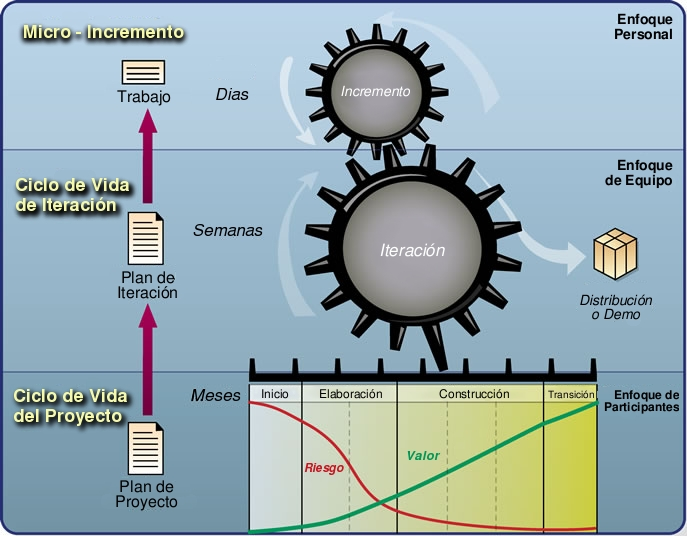
\includegraphics[width=10cm]{planificacion/iteracionIncremento}
    \caption{Diferencia entre iteración e incremento.}
    \label{fig:planificacion:iteracionIncremento}
\end{figure}

Es decir, una iteración es un mini-proyecto en el que se obtiene una versión de cada una de las piezas del sistema, sean código o no, y un incremento se puede medir como la diferencia entre una iteración y la anterior.
\newline

El proceso se divide en cuatro partes fundamentales:

\begin{enumerate}

	\item \textbf{Iniciación:} en esta fase se describe el ámbito funcional del sistema, los requisitos de alto nivel y se identifican posibles riesgos. Hay que comprender el sistema y sus límites.

	\item \textbf{Elaboración:} el objetivo principal de esta fase es el de crear la arquitectura básica, para tener una visión de cómo será el sistema completo y además, proponer soluciones a los riesgos identificados.

	\item \textbf{Construcción:} cómo su nombre indica, esta es la fase dónde se construye y prueba la aplicación. Se realiza un pequeño proceso en cascada en cada iteración de esta fase.

	\item \textbf{Transición:} se despliega el sistema y finaliza el proceso.

\end{enumerate}



Cada una de estas fases, como es lógico, puede tener más de una iteración, en función del tamaño del proyecto, con tareas propias de la etapa en que se esté, así por ejemplo, en la etapa de construcción, en cada iteración se escoge un grupo de requisitos de alto nivel, se refinan, y partiendo de la versión del sistema obtenida en la iteración anterior, se diseñan, implementan y prueban esos requisitos, creando la versión que se utilizará en la siguiente iteración.
\newline

Al finalizar el proceso obtenemos tanto el código de la aplicación, como modelos y documentación de la misma que se van creando a lo largo de las iteraciones.
\newline
\todo{añadir imágenes del ciclo de vida}



%Porque se ha escogido

Las principales razones por las que se ha escogido este tipo de proceso y no otro son:

\begin{itemize}

	\item[\ding{70}] Poca incertidumbre a la hora de diseñar y planificar, ya que al realizarse en cada iteración y no del sistema completo, se tiene mayor comprensión de los riesgos y de las tareas a realizar.

	\item[\ding{70}] Se adapta bien a cambios de requisitos.

	\item[\ding{70}] Si se priorizan los requisitos para implementarlos en las primeras iteraciones de la construcción, se obtiene una aplicación con funcionalidades clave en la que el cliente puede decidir si está o no correcto.

	\item[\ding{70}] Al trabajar con un subconjunto de requisitos en cada iteración la complejidad se reduce, lo que facilita que se reduzca también el número de errores producidos.

\end{itemize}


\begin{figure}[!htb]
    \centering
    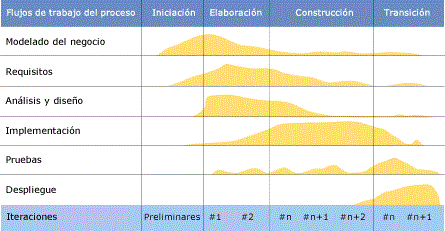
\includegraphics[]{planificacion/trabajoFases}
    \caption{Carga de trabajo en las diferentes fases.}
    \label{fig:planificacion:trabajoFases}
\end{figure}


De la primera fase, \emph{iniciación}, la descripción funcional detallando el alcance del sistema está descrita en la sección \ref{sec:planificacion:descFuncional}, a continuación se muestra un diagrama de casos de uso, basado en esa descripción y en la siguiente sección se describen los requisitos de alto nivel extraídos.

\begin{figure}
    \centering
    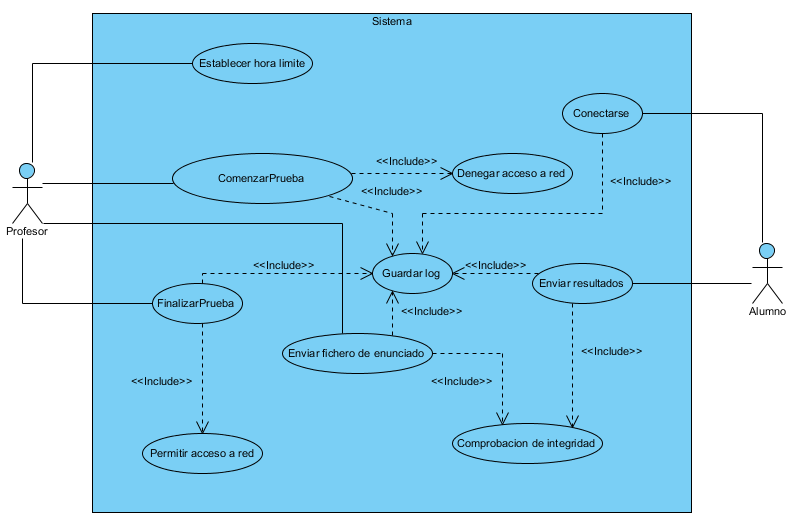
\includegraphics[width=10cm]{planificacion/casosUsoSistema}
    \caption{Diagrama de casos de uso del sistema}
    \label{fig:planificacion:casosUso}
\end{figure}



\section{Requisitos de Alto Nivel del Sistema}
\label{sec:planificacion:requisitos}

%==========================================================================%
% NOTA(Pablo): Ligando las secciones, que siempre queda muy bien
%==========================================================================%
Esta sección describe el segundo paso en nuestro proceso de desarrollo, de acuerdo a la metodología descrita en la sección anterior, que es la identificación de los requisitos de alto nivel que ha de satisfacer nuestro sistema software, de acuerdo a la descripción del ámbito funcional proporcionada en la Sección~ \ref{sec:planificacion:descFuncional}.
\newline
%==========================================================================%
% NOTA(Pablo): Todo esto se considera sabido, por lo que no hay que
%              escribirlo
%==========================================================================%
% Definirlas de modo correcto es muy importante, ya que los requisitos de
% alto nivel dependen directamente y si estos son incorrectos, obtendríamos
% una aplicación inútil que no cumple con lo requerido.
%
% Un requisito es una propiedad que debe ser exhibida por un software para
% resolver un problema particular.
% Los requisitos han de tener ciertas características, entre ellas ser:
% \begin{itemize}
%    \item \emph{No ambiguos,} no puede haber varias interpretaciones para un %requisito puesto que se puede optar por una solución no deseada por el cliente.
%
%\item \emph{Entendible,} se comprende fácilmente el significado.
%
%\item \emph{Verificable,} es necesario que existan técnicas para comprobar que cada requisito es construido correctamente.
%
%\end{itemize}
%El conjunto de requisitos ha de ser, entre otras cosas:
%
%\begin{itemize}
%
%\item \emph{Completo,} de tal forma que todo lo que deba hacer la aplicación está recogido.
%\item \emph{Consistente,} no deben existir conflictos entre requisitos.
%\item \emph{No redundante,} es decir, que un problema sólo lo resuelva un único requisito.
%
%\end{itemize}

En concreto, se han identificado los siguientes requisitos de alto nivel para nuestro sistema

\todo {arreglar la tabla}

\begin{table}
\begin{tabular}{|c|l|}
	\hline
	\textbf{Identificador} & \textbf{Descripción}
	\\ \hline

	R01 & Un computador de la red debe poder ser designado como \emph{Watchman}.
	\\ \hline

	R02 & Todos los computadores que no sean \emph{Watchman} serán computadores
	normales, y podrán ser utilizados para la realización de las pruebas evaluables.
	\\ \hline

	R03 & El profesor debe ser capaz desde el \emph{Watchman} de indicar el inicio de la prueba.
	\\ \hline

	R04 & El profesor debe ser capaz desde el \emph{Watchman} de indicar el fin de la prueba.
	\\ \hline

	R05 & El profesor ha de ser capaz desde el \emph{Watchman} de establecer una hora límite para la duración de la prueba.
	\\ \hline

	R06 & El profesor debe ser capaz desde el \emph{Watchman} de enviar el fichero de enunciado al resto de computadores.
	\\ \hline

	R07 & El alumno desde su computador debe ser capaz de conectarse al \emph{Watchman}.
	\\ \hline

	R08 & El alumno desde su computador debe ser capaz de enviar sus resultados al profesor.
	\\ \hline

	R09 & El alumno desde su computador debe ser capaz de indicar que da por finalizada la prueba.
	\\ \hline

	R10 & El alumno desde su computador debe tener la posibilidad de ver el tiempo restante el pruebas de duración prefijada.
	\\ \hline

	R11 & La aplicación del alumno ha de ser capaz de denegar el acceso a la red al empezar la prueba.
	\\ \hline

	R12 & La aplicación del alumno ha de ser capaz de permitir el acceso a la red al finalizar la prueba.
	\\ \hline

	R13 & La aplicación ha de ser capaz de comprobar que los archivos se han enviado correctamente.
	\\ \hline

	R14 & La aplicación del profesor ha de ser capaz de guardar registros de actividad.
	\\ \hline

\end{tabular}
\label{tabla:requisitos}
\caption{Requisitos del sistema}
\end{table}

\section{Iteraciones}

En esta sección se describen las iteraciones previstas para el desarrollo de la aplicación.

\begin{itemize}
    \item {\bfseries Iteración 1: Crear un sistema distribuido.}
    \begin{itemize}
        \item Requisitos implementados: R06, R07
        \item Descripción: En la primera iteración la aplicación del alumno se podrá conectar al watchman para esperar el inicio de la prueba, envío de ficheros etc... y el profesor es capaz de enviar el enunciado.
    \end{itemize}

    \item {\bfseries Iteración 2: Denegar acceso a red una vez comenzado el examen.}
    \begin{itemize}
        \item Requisitos implementados: R03, R05, R10, R11
        \item Descripción: En la segunda iteración el profesor puede establecer una hora límite e indicar el inicio de la prueba. La aplicación del alumno es capaz de denegar el acceso a la red cuando se inicia la prueba y en caso de que la duración este prefijada, consultar el tiempo restante
    \end{itemize}


    \item {\bfseries Iteración 3: Habilitar red y enviar resultados}
    \begin{itemize}
        \item Requisitos implementados: R04, R08, R09, R12
        \item Descripción: En la tercera iteración se permite al profesor finalizar la prueba de modo general. Del mismo modo, cada alumno puede finalizar la prueba por su cuenta y enviar su archivo de resultados al computador del profesor. La aplicación del alumno, cuando este finaliza la prueba, habilita el acceso a la red.
    \end{itemize}


    \item {\bfseries Iteración 4: Comprobación de integridad}
    \begin{itemize}
        \item Requisitos implementados: R13
        \item Descripción: En la cuarta iteración se implementa el sistema de comprobación de integridad de los ficheros transmitidos por red para garantizar la correcta recepción de los mismos.
    \end{itemize}

    \item {\bfseries Iteración 5: Sistema de logs}
    \begin{itemize}
        \item Requisitos implementados: R14
        \item Descripción: Definir los mensajes necesarios para cuando en la aplicación ocurre algo que se desee guardar.
    \end{itemize}
\end{itemize}


En cuanto a los requisitos R01 y R02 están implementados en arquitectura del sistema, no son funcionalidades.
\newline

En este capítulo se ha descrito el ámbito funcional del sistema y la metodología a utilizar para desarrollarlo. De acuerdo a este plan de desarrollo, se han obtenido los requisitos y planteado una serie de iteraciones a seguir para la construcción de la aplicación.
\newline


% Los requisitos R01 y R02 están implementados en arquitectura del sistema, no son
% funcionalidades.


%Iteraciones previstas

% Iteración 1: Crear un minisistema distribuido
%R06, R07 - En la primera iteración la aplicación del alumno se podrá conectar al watchman para esperar el inicio de la prueba, envío de ficheros etc... y el profesor es capaz de enviar el enunciado.

% Iteración 2: Denegar acceso a red una vez comenzado el examen
%R03, R05, R10, R11 - En la segunda iteración el profesor puede establecer una hora límite e indicar el inicio de la prueba. La aplicación del alumno es capaz de denegar el acceso a la red cuando se inicia la prueba y en caso de que la duración este prefijada, consultar el tiempo restante


%Iteración 3: Habilitar red y enviar resultados
%R04, R08, R09, R12 - En la tercera iteración se permite al profesor finalizar la prueba de modo general. Del mismo modo, cada alumno puede finalizar la prueba por su cuenta y enviar su archivo de resultados al computador del profesor. La aplicación del alumno, cuando este finaliza la prueba, habilita el acceso a la red.

% Los requisitos R01 y R02 están implementados en arquitectura del sistema, no son
% funcionalidades.

% Iteración 4:
% R13: Se implementa tanto en el caso de que el profesor envíe el enunciado, como cuando reciba % los resultados.

% Iteración 5:
% R14: Cuando en la aplicación ocurre algo de lo que se deseen guardar logs se implementará con % independencia de la iteración en la que nos encontremos.




% Cap\'itulo 3: Resumen del Estado del Arte
%==================================================================%
% Author : Pando Muñoz, Manuel                                     %
%          Sánchez Barreiro, Pablo                                 %
% Version: 1.0, 02/03/2011                                         %
%                                                                  %
% Memoria del Proyecto Fin de Carrera                              %
% Archivo raíz para el capítulo de antecedentes                    %
%==================================================================%


\chapterheader{Antecedentes}{Antecedentes}
\label{chap:introduction}

%==================================================================%
% TODO(Pablo) : Completa este párrafo introductorio de manera      %
%               adecuada                                           %
%==================================================================%

El siguiente cap\'itulo describe brevemente las tecnolog\'ias sobre las que se fundamenta el presente proyecto. M\'as concretamente, se explica el funcionamiento de las redes locales, del framework Netfilter para el filtrado de paquetes, y de los demonios en los sistemas Linux, tres aspectos fuertemente relacionados con el proyecto. \newline

La aplicación a desarrollar está pensado que se utilice en los laboratorios de la Facultad de Ciencias de la Universidad de Cantabria, en estos laboratorios los computadores están conectado mediante una \emph{red local} y utilizan sistemas Linux. Para gestionar los permisos de acceso a la red se va a utilizar un \emph{demonio} que interactúe con \emph{Netfilter} por medio de iptables.


\chaptertoc

\section{Red local}

%============================================================================%
% NOTA(Pablo): Poner un párrafo de como se ha llegado hasta aquí             %
%============================================================================%
Una Red local o LAN es un conjunto de computadoras conectadas entre sí en un \'area relativamente peque\~na, como los laboratorios de la Facultad.

%============================================================================%
% NOTA(Pablo): Poner ejemplo de área relativamente pequeña y explicar cómo   %
%              y en que se diferencian las LANs de las WANs.                 %
%============================================================================%

Cada uno de estos equipos interconectados en la red se conoce como nodo. Estos nodos son capaces de enviar, recibir y procesar comandos con el fin de transportar datos, así como compartir informaci\'on y recursos a través de la red.

%============================================================================%
% NOTA(Pablo): Esto queda suelto                                             %
%============================================================================%
El funcionamiento de la red está estandarizado siendo el protocolo TCP/IP el más extendido.

%============================================================================%
% NOTA(Pablo): Esto suena a escribir por escribir, así que mejor lo quitamos %
%============================================================================%
% Entre las ventajas de las redes locales cabe destacar el ahorro en hardware,
% si se desea que todos los equipos puedan imprimir no es necesario disponer de % una impresora para cada equipo, sirve con una conectada a la red, y del mismo % modo, el ahorro en la factura de internet, puesto que con una sola conexi\'on % se puede dar acceso a todos los equipos de la red.
%
% Otra ventaja, probablemente la m\'as importante desde el punto de vista
% t\'ecnico es que al estar estandarizados como han de comunicarse los nodos en % la red permite la conexi\'on de equipos heterog\'eneos.
%============================================================================%

%==================================================================%
% TODO(Pablo) : Esto así a pelo queda muy duro, quizás haya que    %
%               explicar antes cómo es la arquitectura global de   %
%               la aplicación.                                     %
%==================================================================%

\section{Daemon}

% NOTA(Pablo): No se suele decir la palabra "informática", ya que está
%              demasiado sobrecargada y no se sabe si son redes,
%              programación, inteligencia artificial o simplemente saber
%              manejar el Word
% En inform\'atica

Un \emph{demonio} (del inglés, \emph{daemon}) es un tipo de proceso que posee la siguientes características:

\begin{enumerate}
	\item Se ejecuta en segundo plano;
	\item Generalmente se inicia en tiempo de arranque;
	\item No usa los sistemas de entrada/salida est\'andar;
	\item Mantienen la información que necesitan en ficheros especiales bien identificados.
\end{enumerate}

%=========================================================================%
% NOTA(Pablo): Esta información es demasiado técnica y poco interesante.  %
%              Mejor la borramos                                          %
%=========================================================================%
% En los sistemas Windows se conocen como servicios ya que son usados para,
% precisamente, proporcionar un servicio al usuario.
% En los sistemas linux, cada daemon suele tener un script en la carpeta
% /etc/init.d/ que permite iniciarlo, pararlo o consultar su estado.
%
% El nombre del ejecutable suele acabar en "d".
%
%=========================================================================%

Normalmente est\'an cargados en memoria esperando una se\~nal para ser ejecutados, por lo que su gasto de recursos no suele ser significativo.

% NOTA(Pablo): Pero consumen memoria, ¿no?

%=========================================================================%
% NOTA(Pablo): Esta información es demasiado técnica y poco interesante.  %
%              Mejor la borramos                                          %
%=========================================================================%
%
% Adem\'as suelen ser concurrentes, es decir, cuando se va a atender una
% petici\'on, el daemon crea un hilo especifico para ejecutar las \'ordenes de
% esa petici\'on concreta, de modo que el hilo principal puede seguir a la
% espera de nuevas peticiones.\newline
%
%=========================================================================%

%=========================================================================%
% NOTA(Pablo): Faltaría poner un ejemplo de demonio y dejar clara su      %
%              utilidad, sin entrar en detalles técnicos                  %
%              Habría que poner también la utilidad de los demonios para  %
%              el proyecto en cuestión                                    %
%=========================================================================%

%=========================================================================%
% NOTA(Pablo): Titular la sección con el nombre del concepto que          %
%              representan las ip tables                                  %
%=========================================================================%

\section{Netfilter : Iptables}

%=========================================================================%
% NOTA(Pablo): Esto sin ningún tipo de intoducción, así a bocajarro,      %
%              queda un poco duro                                         %
%=========================================================================%

Netfilter es un framework que permite filtrar de paquetes, traducci\'on de direcciones y puertos de red y varias funcionalidades m\'as para el manejo de paquetes. Es parte del n\'ucleo de linux desde la versi\'on 2.4 del mismo, sustituyendo a ipchains, bastante limitado en comparaci\'on con Netfilter.

%=========================================================================%
% NOTA(Pablo): Demasiado técnico y poco interesante, lo borramos          %
%=========================================================================%
% Iptables es una aplicaci\'on de l\'inea de comandos, que permite a un
% usuario con privilegios de administrador, configurar un conjunto de
% reglas para el filtrado de paquetes.
%
%  Tambi\'en es parte del mismo proyecto que Netfilter, por lo que
% generalmente se suele hablar solamente de iptables, puesto que es el
% programa con el que interact\'ua directamente el usuario, para referirse
% al d\'uo netfilter/iptables.
%

Ejemplo de uso de iptables
\begin{center}
\# iptables -A INPUT -s 195.65.34.234 -j ACCEPT\\
\end{center}

El par\'ametro -A indica que se va a a\~nadir una regla, el objetivo de la mismo es aceptar todos los paquetes entrantes provenientes del host indicado\footnote{en vez de la IP podemos poner su FQDN (\emph{Fully Qualified Domain Name) sin lo desearamos}. Del mismo modo, si lo que queremos es no aceptar las peticiones se cambiar\'ia ACCEPT por DROP y si nos queremos referir a los paquetes salientes OUTPUT por INPUT.}
%============================================================================%
% NOTA(Pablo): Por defecto ¿qué pasa cuando un paquete                       %
%              proviniente de un host llega y no se ha tocado iptables?      %
%              ¿Se rechaza o se acepta?                                      %
%============================================================================%



% Cap\'itulo 4: Definici\'on Arquitect\'onica y Dise\~no Software
%==================================================================%
% Author : Pando Muñoz, Manuel                                     %
%          Sánchez Barreiro, Pablo                                 %
% Version: 1.0, 30/03/2011                                         %
%                                                                  %
% Memoria del Proyecto Fin de Carrera                              %
% Archivo raíz para el capítulo de la arquitectura del sistema     %
%==================================================================%


\chapterheader{Arquitectura y diseño}{Definición Arquitectónica y Diseño Software}
\label{chap:arquitectura}

En el presente capítulo se presentan, mediante diagramas UML, la arquitectura física del sistema, los módulos y las comunicaciones entre ellos existentes en el sistema, y el funcionamiento del mismo.

 \todo{finalizar breve introducción}

\chaptertoc

\section{Arquitectura física del Sistema}
\label{sec:arquitectura:arqFisica}

En esta sección se describe la arquitectura física del sistema mediante un diagrama de despliegue.
\begin{figure}
    \centering
    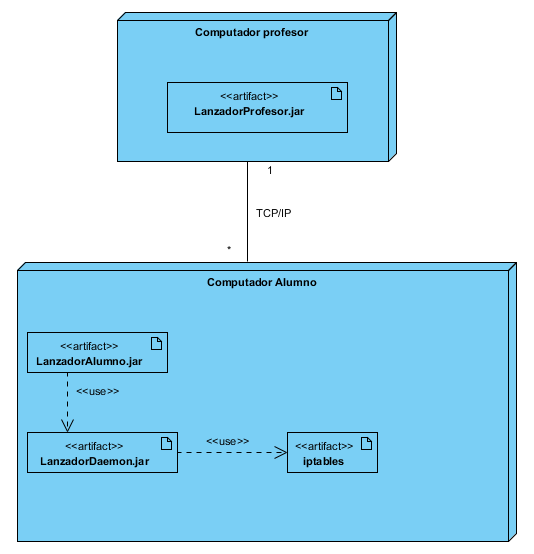
\includegraphics[width=.75\linewidth]{arquitectura/despliegueSistema}
    \caption{Diagrama de despliegue del sistema}
    \label{fig:arquitectura:despliegueSistema}
\end{figure}
\newline


\lq\lq LanzadorProfesor.jar\rq\rq contiene lo necesario para mostrar la interfaz de usuario en la aplicación del profesor, así como la lógica de manejo de eventos y comunicación con las aplicaciones de los alumnos.

\lq\lq LanzadorAlumno.jar\rq\rq contiene las funciones para mostrar la interfaz de usuario de la aplicación del alumno, el manejo de eventos producidos por su uso y la lógica de comunicación con la aplicación del profesor y el demonio local.

\lq\lq LanzadorDaemon.jar\rq\rq contiene la lógica de comunicación con la aplicación del alumno y lo necesario para interactuar con iptables.

\lq\lq iptables\rq\rq es parte del núcleo del sistema Linux sobre el que se ejecutará la aplicación.

Cómo se puede puede observar, sólo se permite la existencia de una aplicación en el computador del profesor, a la que se conectan mediante TCP/IP un número indefinido de aplicaciones alumno, lógico, ya que en cada prueba suele haber varios los alumnos realizándola y uno el número de profesores.
\newline

A su vez, la aplicación del alumno interactúa con un único demonio del sistema.


\section{Diseño Software}
\label{sec:arquitectura:diseno}

En está sección se muestra un diagrama de actividad que resume las posibles interacciones que tanto el alumno como el profesor realizan con sus respectivas aplicaciones durante el trascurso normal de una prueba.
\newline

\begin{figure}
    \centering
    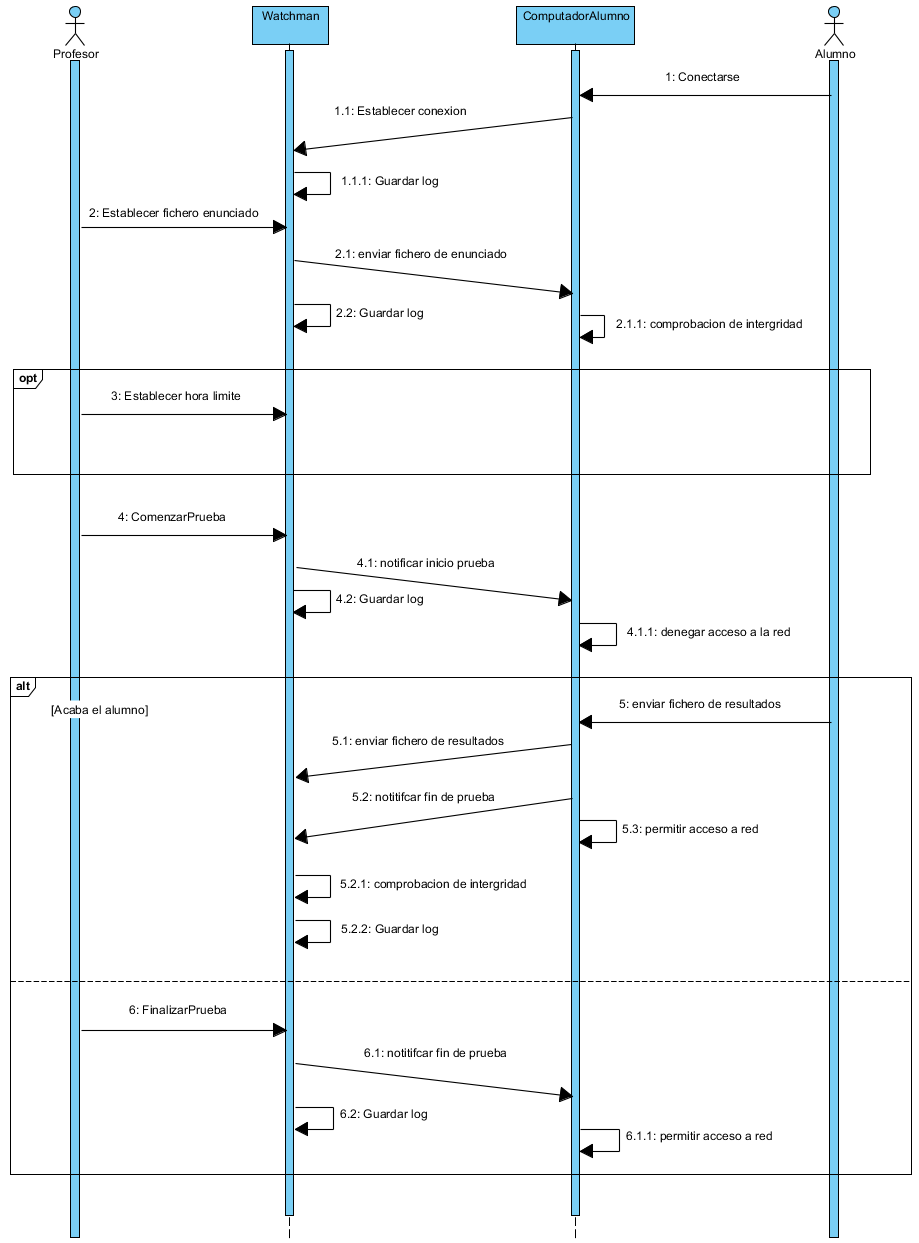
\includegraphics[width=12cm]{arquitectura/actividadSistema}
    \caption{Diagrama de actividad del sistema}
    \label{fig:arquitectura:actividadSistema}
\end{figure}


Vemos que se siguen los pasos descritos en la sección \ref{sec:planificacion:descFuncional}


%% Razonar porque el software es seguro
La principal funcionalidad de la aplicación es la de denegar el acceso a la red en los computadores de los alumnos que están realizando la prueba, mientras la prueba esté en marcha, sin necesidad de apagar el router o switch del laboratorio. Esto se consigue por medio de iptables, cambiando la política de los paquetes salientes una vez que empieza la prueba y hasta que acaba.
\newline

Por defecto iptables permite todo el tráfico que entre y salga del equipo, modificando las reglas para que deseche cualquier paquete destinado a cualquier equipo, conseguimos que no se pueda realizar ninguna petición a ningún nodo de la red, y, por tanto, tampoco recibiremos el contenido de la posible respuesta, el equipo del alumno queda aislado del resto.
\newline

A la hora de volver a permitir el acceso a la red, basta con modificar la política para el tratamiento de los paquetes salientes y restaurarla al estado anterior. Un alumno corriente no puede realizar esta operación ya que son necesarios privilegios de administrador para ello.
\newline

Otro punto importante es el de la recogida de resultados automática, se ha de garantizar que el archivo no se ha corrompido a lo largo de la transferencia, para ello se realizan, tanto en el equipo que envía el fichero como en el que lo recibe, firmas MD5 al mismo para comprobar que no ha habido errores en la transferencia.


\begin{figure}
    \centering
    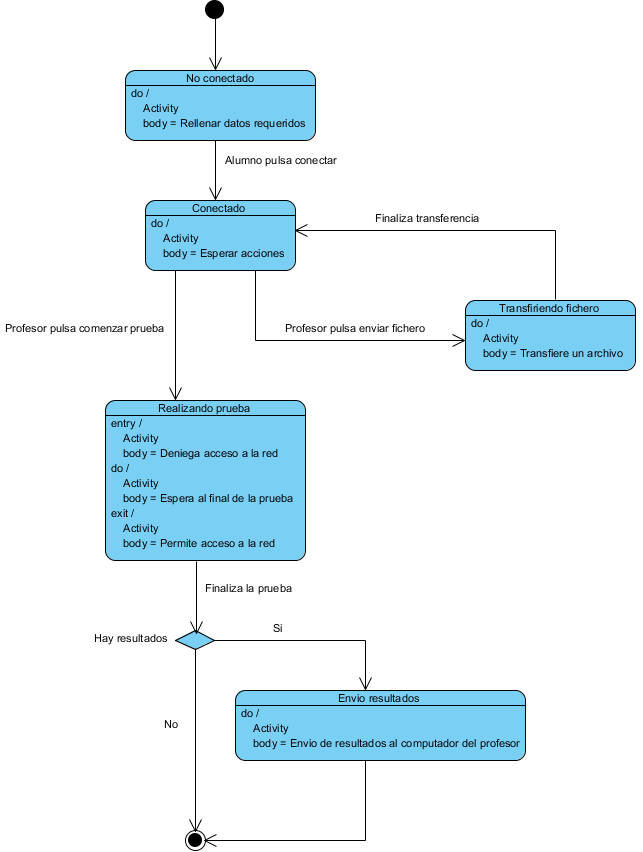
\includegraphics[width=12cm]{arquitectura/estadosAlumno}
    \caption{Diagrama de estados de la aplicación del alumno}
    \label{fig:arquitectura:estadosAlumno}
\end{figure}


En la figura \ref{fig:arquitectura:estadosAlumno} se describen los estados por los que puede pasar la aplicación del alumno. Se corresponden directamente con el estado en que se encuentra la prueba. 

%% Describir la arquitectura física del sistema (despliegue)

%% Diagrama de secuencia general del sistema

%% Estados del ordenador del alumno

%% Razonar porque el software es seguro

% Capítulo 5: Ejemplo de una iteración
%==================================================================%
% Author : Pando Muñoz, Manuel                                     %
%          Sánchez Barreiro, Pablo                                 %
% Version: 1.0, 02/03/2011                                         %
%                                                                  %
% Memoria del Proyecto Fin de Carrera                              %
% Archivo raíz para el capítulo de iteración                       %
%==================================================================%

\chapterheader{Segunda iteración}{Descripción de una iteración}
\label{chap:iteracion}

\chaptertoc

En el siguiente capítulo se describe lo realizado en la segunda iteración de construcción.
Se parte de lo obtenido en las iteraciones previas, que es, la descripción del sistema, la arquitectura del mismo y los diagramas de secuencia y estados, todo esto expuestos a lo largo de los capítulos \ref{chap:planificacion} \ref{chap:arquitectura}.
En cuanto al estado de la aplicación, en la primera iteración de construcción se ha desarrollado un sistema distribuido, en el que desde la aplicación del alumno se puede conectar con la aplicación del profesor y transmitir ficheros.
El objetivo de esta iteración es que el profesor pueda establecer el inicio y de la prueba, poder prefijar una hora de finalización de la misma y que la aplicación del alumno sea capaz de denegar el acceso a la red mientras dure la prueba. %
En las siguientes secciones se describen los incrementos realizados dentro de esta iteración.

%contar el desarrollo del daemon
%contar como utilizo iptables
%Secciones: Inicio de prueba, Examen temporizado, Denegar acceso red

\section{Inicio de la prueba}
\label{sec:iteracion:iniPrueba}

En esta sección se comenta cómo se consigue que el profesor pueda notificar a los alumnos el inicio de la prueba.
Como ya hemos comentado, partimos de la iteración anterior en la cual los alumnos eran capaces de conectar a la aplicación del profesor. En la aplicación del alumno, cuando se crea una conexión, se inicia a su vez un hilo de ejecución que se mantiene a la espera de recibir distintas órdenes provenientes del computador del profesor. De este modo se hace muy simple mantener desde la aplicación del profesor una lista de las conexiones abiertas con cada alumno y, al presionar el botón de iniciar la prueba, recorrer esa lista enviando la orden por cada conexión.

Cuando cada una de las aplicaciones del alumno recibe esa orden, actúa en consecuencia.

\section{Examen temporizado}
\label{sec:iteracion:examenTemporizado}

El profesor puede establecer una hora límite, llegada la cual, la prueba terminará automáticamente. Cuando el profesor define este límite en su aplicación y decide comenzar la prueba se envía también si hay una hora de fin y, en caso afirmativo, cual es. De este modo la aplicación del alumno puede mostrar una cuanta atrás con los minutos restantes para la finalización, para facilitar la referencia temporal. Se puede ver el resultado en la siguiente imagen.

\begin{figure}[!htb]
    \centering
    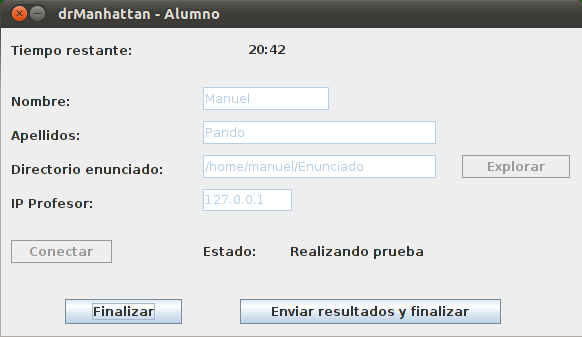
\includegraphics[width=.75\linewidth]{iteracion/tiempoRestante}
    \caption{Aspecto de la GUI del alumno con una prueba temporizada.}
    \label{fig:iteracion:tiempoRestante}
\end{figure}


\section{Denegar acceso a red}
\label{sec:iteracion:denegarRed}

Cómo ya hemos visto en las secciones anteriores, una vez que la aplicación del alumno recibe la orden de comenzar la prueba, se ha de denegar el acceso a la red. Para ello se utiliza iptables, por medio de un demonio.

El demonio creado es muy simple, se ejecuta en segundo plano esperando a que la aplicación del alumno conecte, y en función de lo requerido en ese momento, permitir o no el acceso a la red interactuando con iptables. Este demonio se inicia en tiempo de arranque y con los permisos necesarios para poder usar el cortafuegos.


\section{Pruebas}
\todo{tema seguridad de que no se puede acceder a red}


%% Describe la que más te guste

% Cap\'itulo 6: Construcci\'on, Implementaci\'on, Pruebas y Despliegue

%% Detalles de implementación

%==================================================================%
% Author : Pando Muñoz, Manuel                                     %
%          Sánchez Barreiro, Pablo                                 %
% Version: 1.0, 10/06/2011                                         %
%                                                                  %
% Memoria del Proyecto Fin de Carrera                              %
% Archivo raíz para el capítulo de implementación                  %
%==================================================================%

\chapterheader{Despliegue y aceptación}{Despliegue y aceptación}
\label{chap:despliegue}

\chaptertoc

\todo{introducción}



\section{Despliegue}
\label{sec:despliegue:despliegue}

Para que la aplicación pueda ser probada de un modo cómodo fuera del ambiente de desarrollo se hace necesaria la creación de instaladores. Esto se puede hacer, por ejemplo, con el comando \emph{dpkg} en sistemas Linux derivados de Debian, ya que con el se crear archivos .deb. En nuestro caso se han de crear dos instaladores, uno para la aplicación del profesor, y otro para la aplicación de los alumnos.
\newline

En el sistema de archivos, cada carpeta tiene su utilidad, conocida por todos, de modo que si, por ejemplo, queremos conocer los logs generados por alguna aplicación sabemos que hemos de buscar en /var/log/, /etc/ para los temas de configuraciones, etc.
\newline

Esto es interesante conocerlo para que los archivos que coloque nuestro instalador en el sistema, estén correctamente ubicados, de modo que se puedan localizar fácilmente, en caso de querer modificarlos o eliminarlos.
\newline

Por ejemplo, la aplicación del alumno, creará en los siguientes directorios, los siguientes ficheros:

\begin{itemize}

    \item {\bfseries /etc/rc2.d:}
    \begin{itemize}
        \item \emph{S88drManhattanDaemon}
    \end{itemize}

    Este fichero contiene un script muy simple que se encarga de iniciar en segundo plano el demonio. Los ficheros en este directorio se ejecutan cuando se entra al segundo nivel de ejecución, en el arranque del sistema.


    \item {\bfseries /usr/bin:}
    \begin{itemize}
        \item \emph{drManhattanAlumno.jar}
        \item \emph{drManhattanAlumno.sh}
        \item \emph{drManhattanDaemon.jar}
    \end{itemize}

    En este directorio se encuentran los ejecutables de las aplicaciones que pueden utilizar todos los usuarios.

    \item {\bfseries /usr/share/applications:}
    \begin{itemize}
        \item \emph{drManhattanAlumno.desktop}
    \end{itemize}

    En nuestro caso se ha utilizado un sistema Ubuntu con el entorno de escritorio GNOME, en ese directorio se guardan las entradas de cada aplicación que se puede ejecutar en GNOME, en archivos de texto dónde se especifica la ruta del ejecutable, el icono del programa, su versión, comentarios, etc.


    \item {\bfseries /usr/share/drManhattanAlumno/iconos:}
    \begin{itemize}
        \item \emph{icono.png}
        \item \emph{envioFichero.png}
        \item \emph{explorar.png}
        \item \emph{fin.png}
    \end{itemize}

    Contiene los datos que no dependen de la arquitectura del sistema, imágenes, sonidos, etc.

    \item {\bfseries /usr/share/menu:}
        \begin{itemize}
            \item \emph{drManhattanAlumno}
        \end{itemize}

    Cada archivo localizado en este directorio contiene la información necesaria para que GNOME pueda crear una entrada en el menú despegable de aplicaciones.

    \todo{añadir los fichero de doc, licencia}

\end{itemize}



Una vez que están definidos los archivos y el directorio dónde los ha de colocar el instalador, creamos una carpeta a modo de raíz en la que simulamos el árbol de directorios anterior. Por ejemplo, creamos la carpeta /home/usuario/deb, y dentro de ella creamos /home/usuario/deb/etc/rc2.d/, /home/usuario/deb/usr/bin/, etc y los archivos correspondientes.
\newline

Dentro de la carpeta raíz se ha de crear además de lo anterior, un directorio llamado \"DEBIAN\" con tres ficheros, "control", "postinst" y "postrm". En el primero se especifican las características del paquete y los otros dos se ejecutan justo después de instalar el paquete y justo después de desinstalarlo, respectivamente, en nuestro caso actualizan los menús desplegables para que aparezca o desparezca la aplicación.
\newline

Una vez que tenemos todo creado, cambiamos los permisos del directorio raiz y subdirectorios así:

\begin{center}
    \emph{chown root.root -R /home/usuario/deb/}
\end{center}

Después de esto, la orden para empaquetarlo en un fichero .deb es:

\begin{center}
    \emph{dpkg -b /home/usuario/deb /home/usuario/paquete.deb}
\end{center}

Para instalar, teniendo permisos de administrador:

\begin{center}
    \emph{dpkg -i /home/usuario/paquete.deb}
\end{center}


%Listado de pruebas


\section{Pruebas}
\label{sec:despliegue:pruebas}

Como se comentó en la sección \ref{sec:iteracion:pruebas} en la que se explicaban las pruebas realizadas durante una iteración, las pruebas han sido combinaciones de acciones, tanto de modo local mientras se desarrollaba, como en los laboratorios de la Facultad con el objetivo de imprimir mayor realismo en el entorno de ejecución como la carga de las aplicaciones.
\newline

\todo{poner el resultado y el resultado esperado en cada prueba}

\begin{enumerate}

    \item Intentar conectar a una IP en la que no se está ejecutando la aplicación del profesor.

    \item Sin alumnos conectados, enviar fichero de enunciado.

    \item Con un alumno conectado, enviar ficheros de enunciado.

    \item Con varios alumnos conectados, enviar ficheros de enunciado.


    \item Iniciar prueba sin alumnos conectados.

    \item Iniciar prueba con varios alumnos conectados.


    \item Introducir hora errónea e iniciar prueba.

    \item Iniciar prueba temporizada y esperar a que acabe el tiempo.

    \item Iniciar prueba temporizada y finalizar manualmente.


    \item Iniciar prueba normal y finalizar todos los alumnos sin resultados.

    \item Iniciar prueba normal y finalizar alumnos sin resultados y alumnos con ellos.

    \item Iniciar prueba normal y finalizar todos los alumnos con resultados.

    \item Iniciar prueba normal y finalizar mientras hay alumnos realizando la prueba.



    \item Iniciar prueba normal y reiniciar el computador de un alumno para intentar reconectar sin acabar la prueba.

    \item Iniciar prueba normal, reiniciar el computador de un alumno, finalizar la prueba e intentar reconectar.



    \item Iniciar prueba temporizada y reiniciar el computador de un alumno para reconectar antes de que se acabe la prueba.

    \item Iniciar prueba temporizada y reiniciar el computador de un alumno para reconectar después de que se acabe la prueba.

\end{enumerate}


Esta lista contiene las pruebas de integración y validación realizadas, esto es, cuándo se prueba el funcionamiento del sistema completo para comprobar que cumple los requisitos establecidos en la tabla \ref{tabla:requisitos}.
\newline



% Cap\'itulo 7: Discusi\'on, Conclusiones y Trabajos Futuros

%%==================================================================%
% Author : Pando Muñoz, Manuel                                     %
%          Sánchez Barreiro, Pablo                                 %
% Version: 1.0, 10/06/2011                                         %
%                                                                  %
% Memoria del Proyecto Fin de Carrera                              %
% Archivo raíz para el capítulo de Conclusiones y trabajos futuros %
%==================================================================%


\chapterheader{Discusi\'on, Conclusiones y Trabajos Futuros}{Discusi\'on, Conclusiones y Trabajos Futuros}
\label{chap:futuro}

\section{Conclusiones}
\label{sec:futuro:conclusiones}

Como se comentaba al principio de este documento el objetivo del proyecto era el de crear una aplicación que facilitase la realización de pruebas evaluables a los docentes, automatizando ciertas tareas que sino han de realizarse manualmente, como la recogida de resultados, con el gasto de tiempo que ello conlleva, además de tener que ser realizado secuencialmente.
\newline

Para conseguir esto, se ha pasado por una fase de investigación, para tener conocimientos suficientes del problema a solucionar, las diferentes opciones posibles para ello y poder así tomar decisiones razonadas. Esto se transformó en una planificación y un diseño del proyecto, que se ha ido exponiendo a lo largo del documento.
\newline

La solución obtenida es una aplicación Open Source que permite, enviar archivos desde el computador del profesor a los alumnos, deshabilitar el acceso a la red durante el transcurso de la prueba, haciendo uso de iptables, software muy utilizado y probado, recoger automáticamente los resultados, comprobando la integridad de los ficheros, como principales funciones a través de interfaces visuales intuitivas y amigables.
\newline


Una de las lecciones que considero más importantes aprendidas a lo largo del desarrollo de este proyecto de fin de carrera, es la importancia de tener unos requisitos claros y definidos antes de planificar el diseño y construcción de la aplicación y tener un análisis y un diseño correcto y claro antes de codificar realmente el software y cómo el cambio en requisitos en fases avanzadas del proyecto puede suponer muchas horas de trabajo extra, en comparación con las primeras fases.
\newline

Merece la pena \lq\lq perder\rq\rq \ el tiempo revisando los requisitos y sus posibles incongruencias antes de empezar con la codificación.
\newline


Durante la realización de las pruebas descritas en la sección \ref{sec:implementacion:pruebas} se encontraba presente el administrador de sistemas de la Facultad, que propuso la funcionalidad de recuperar el estado frente a reinicios del sistema, parecía algo interesante añadirlo a la aplicación, así que se hizo. Esto realmente no significa un cambio en uno de los requisitos, sino la adición de uno nuevo, y gracias a la metodología usada para la construcción, que es flexible y prevé posibles cambios en los requisitos, el tiempo extra de codificación y diseño no fue mucho, comparado con lo que podría haber sido de utilizar una metodología en cascada.
\newline

En la siguiente sección se detallan posibles mejoras o adaptaciones a realizar en la aplicación para aumentar su funcionalidad, usabilidad y atractivo en general.

\section{Trabajos futuros}
\label{sec:futuro:futuro}

Como continuación de este proyecto, en lo referido a su principal función, el mantenimiento de la integridad de las pruebas evaluables, o en el aumento de la comodidad a los docentes, pueden añadirse las siguientes líneas de desarrollo:

\begin{itemize}

    \item {\bfseries Deshabilitar USB:} Los dispositivos USB son otro posible aspecto que podría enturbar los resultados de una prueba, teniendo en cuenta que cada día son mas pequeños.

    \item {\bfseries Acceso restringido:} En algunos momentos puede ser deseable que los alumnos accedan a ciertos contenidos en la red, apuntes de la asignatura en una plataforma como Moodle, por ejemplo, pero no al resto de internet, que el docente pudiese especificar qué contenidos son accesibles y durante cuánto tiempo sin duda puede resultar interesante.

    \item {\bfseries Multiplataforma:} El proyecto ha sido construido íntegramente con el lenguaje de programación Java, pero el hecho de utilizar un cortafuegos propio del sistema Linux hace que no sea multiplataforma. Modificar esa parte del código y adaptarla para otros sistemas, haría que se pudiese utilizar independientemente de la plataforma, algo que es siempre atractivo.

    \item {\bfseries Integración con otras aplicaciones:} Todos sabemos que en lo referente a la seguridad informática no se puede garantizar que una aplicación sea a prueba de todo, la integración con otros sistemas, de análisis de tráfico por ejemplo, proporcionarían un aumento de la confianza en el proyecto.

\end{itemize} 


%%

% CONTENT: Appendices, if desired
%\renewcommand\chaptername{Appendix}                      % hereafter, chapters are called "Appendix"
\renewcommand\thechapter{\Alph{chapter}}        % chapter number in Romans
\renewcommand\thesection{\Alph{chapter}.\alph{section}}  % make sections "I.a", instead of "1.1"
\setcounter{chapter}{0}                                  % start numbering chapters from 1 on again


% Appendix A:
% \input{populo/populo.tex} % Appendix I

% CONFIG: Bibliography style
% \cleardoublepage                            % start in right side page
\addcontentsline{toc}{chapter}{Bibliografía}  % add this "chapter" to the ToC, with the name "Bibliography"
\bibliographystyle{alpha}                  % bibliography style
%\bibliographystyle{abbrv}                  % bibliography style 
% \bibliography{references/references}

\end{document} 